\chapter{Beamformers}\label{ch:beamformers}
\section{Introduction}
In general, a fundamental part of signal processing 
involves filtering in one way or another,
and same is the case for speech signals processing.
The motivation to filter incoming signals 
is to form a given signal so that the unwanted components, 
referred to as interferences, are eliminated,
and the desired component of the signal remains.

A filter can be in the form of an analog or digital circuit. 
In the sense of a fixed-tap or static digital filter, 
the discrete signal samples are tapered 
due to a convolutional multiplication with 
the filter's weighted coefficients.
These coefficients are preset according 
to desired characteristics of the desired output signal.

Since speech signals can vary in tone, pitch, 
formants, and frequencies, statically setting the filter's 
coefficients won't be sufficient 
and robust enough.
To that end the coefficients should be set dynamically
to suit the input signal or the model to be generalized 
to a great end; hence, the filter's performance 
would be suitable for a wide range of inputs rather than
a singular case scenario.
Changing the filter's coefficients dynamically in accordance
with the input or the use case is called ``adaptive filtering''.
In opposed to the case of ``static filtering'' where 
the coefficients are computed once. 

In a case where multiple sources are presented such
as a sensors array, a ``spatial factor'' is introduced
such that the filtered signal is the outcome of
a combination of all the receiving elements
in the array, that maximize the filtering effect.
That ``spatial filtering'' in the presence of
multiple sensors is called ``beamforming''.
The guideline of beamforming is the optimization of
the received signal utilizing all the sensors
to maximize, in most cases, the SNR.
In this research, we show that in E2E-ASR systems,
the introduction of beamformers at the front-end before
the ASR model manifests in higher detection results
and better model accuracy.

The beamforming principle relies on 
acknowledging that the desired signal 
is absorbed and received by multiple sensors 
along with the unwanted interferences. 
In the case of beamforming speech signals, 
the sensors (microphones) are spread in space in 
a dedicated formation and set at a 
known distance from each other.
Each sensor's input can be filtered, delayed, amplified, 
or undergo any form of manipulation 
until eventually summing up with the other sensors' inputs.
In other words, the ability to manipulate each sensor's 
input signal in a multi sensor array gives the ability
to ``form'' a given signal
utilizing the properties of constructive and destructive
interferences. 

We apply the beamforming in the frequency domain: 
\begin{align}
    Y(j\omega) = \mathbf{W}^H(j\omega)\mathbf{X}(j\omega)
\end{align}

The time difference of arrival between 
microphone \(1\) and \(m\) can be estimated 
using the Generalized Cross-Correlation 
with Phase Transform (GCC-PHAT) 
with the following expression:
\begin{align}
\displaystyle\tau_m = argmax_{\tau} \int_{-\pi}^{+\pi}{\frac{X_1(j\omega) X_m(j\omega)^*}{|X_1(j\omega)||X_m(j\omega)|}e^{j\omega\tau}}d\omega
\end{align}

The power corresponds to: 
\begin{align}
    \displaystyle E(\mathbf{u}) = \frac{\mathbf{A}(j\omega,\mathbf{u})^H \mathbf{A}(j\omega,\mathbf{u})}{\sqrt{\mathbf{A}(j\omega,\mathbf{u})^H \mathbf{U}(j\omega)\mathbf{U}(j\omega)^H\mathbf{A}(j\omega,\mathbf{u})}}
\end{align}
The DOA with the maximum power is selected as the DOA of sound:
\begin{align}
    \mathbf{u}_{max} = argmax_{\mathbf{u}}{E(\mathbf{u})}
\end{align}

\section{Multi sensors use-cases}
A multi-microphone array is often named multi-sensors. Every sensor
absorbs the speech differently due to the sensor's spatial location
relatively to the speech source. 
In this work, spacing between sensors and the array's 
formation are pre-known and permanent. 
Knowing the microphone array's shape, 
forming a constructive interference 
is only a matter of the direction of 
arrival since all the other parameters are static.


The human speech frequencies are considered ``long-length'',
which means that the wavelength of the 
frequencies in the audible band is 
between single centimeters to several meters. 
A speaker standing in front of a microphone typically stands 
at a distance that does not exceed several meters, nor is it 
millimeters away. In either situation, the absorbed speech
will be distorted or barely usable. As a result, the propagated speech
waves arrive in a planar shape once they reach the microphone.
In a microphone array, 
these characteristics become handy when applying 
Direction Of Arrival (DOA) and 
Time Difference Of Arrival (TDOA) applications.

A planar wave propagating towards a microphone array 
is depicted in Figure\;\ref{fig:mic_arr_plan}.

\begin{figure}[H]
    \centering
    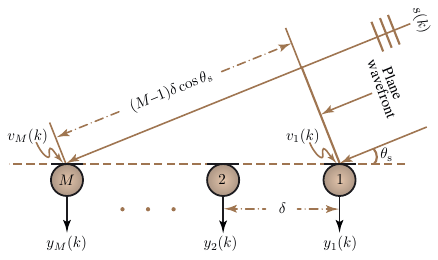
\includegraphics[width=\linewidth]{Beamformers/images/mic_array.png}
    \caption{Microphone array planar wave scenario}\label{fig:mic_arr_plan}
    % \source{Adapted from \citep{MIC_ARRAY}}
\end{figure}

We distinguish between two possible scenarios 
of interest depending on the number 
of sensors and the number of sources.
In one case, multiple connected microphones 
are placed in space, forming a microphone array, 
and in the same space, only a single speaker is present.
The other case is where multiple speakers are present. 
Naming these use cases, we say that a speaker
is referred to as the input to the system, and the microphone array
stands for the system's multiple outputs.
Therefore, we name the single speaker 
scenario a Single Input Multiple Output (SIMO) and the latter 
a Multiple Inputs Multiple Outputs (MIMO).
Demonstrations of these use cases are shown in 
Figures\;\ref{fig:simo_scen} and
\ref{fig:mimo_scen}, respectively.


\begin{figure}[H]
    \centering
    \subfloat[\label{fig:simo_scen}]{%
       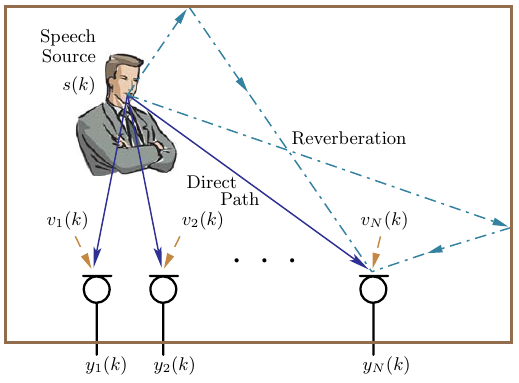
\includegraphics[width=0.45\linewidth]{Beamformers/images/simo_revb_mic_array.png}}
    \hspace{0.1cm}
    \subfloat[\label{fig:mimo_scen}]{%
        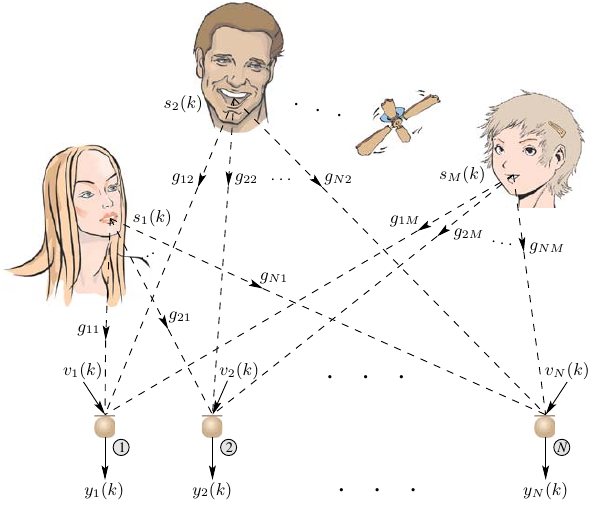
\includegraphics[width=0.45\linewidth]{Beamformers/images/mimo_mic_array_proc.png}}
    \caption{(a) Single Input Multiple Output (SIMO) scenario; (b) Multiple Inputs Multiple Output (MIMO) scenario}
    % \source{Adapted from \citep{ADI_MIMO}}
\end{figure}


\section{Types}

\subsection{Delay-and-Sum}
Delay and sum (DAS) beamformer is a basic beamformer that serves 
as an infrastructure for other beamforming architectures.
These beamformers aim to align the speech part from multiple 
sensors and thus creating the formed beam to conduct 
constructive interference. The speech is then enhanced while 
the other artifacts are attenuated, whether it is ambient noise 
or other unwanted speech from different speakers.

The general architecture for a DAS beamformer is given in Figure\;\ref{fig:das_arch}.
\begin{figure}[H]
    \centering
    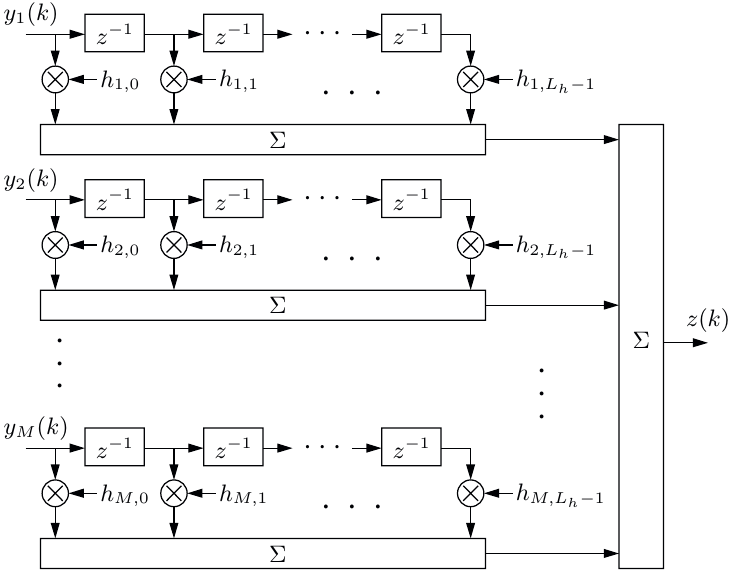
\includegraphics[width=0.85\linewidth]{Beamformers/images/DAS_arch.png}
    \caption{Delay-and-Sum Beamformer architecture}\label{fig:das_arch}
    % \source{Adapted from \citep{ADI_MIMO}}
\end{figure}

Combining the DAS architecture with the microphone array as the input
we get a system capable of dealing with SIMO and MIMO, as shown in
Figure\;\ref{fig:mic_array_proc}.

\begin{figure}[H]
    \centering
    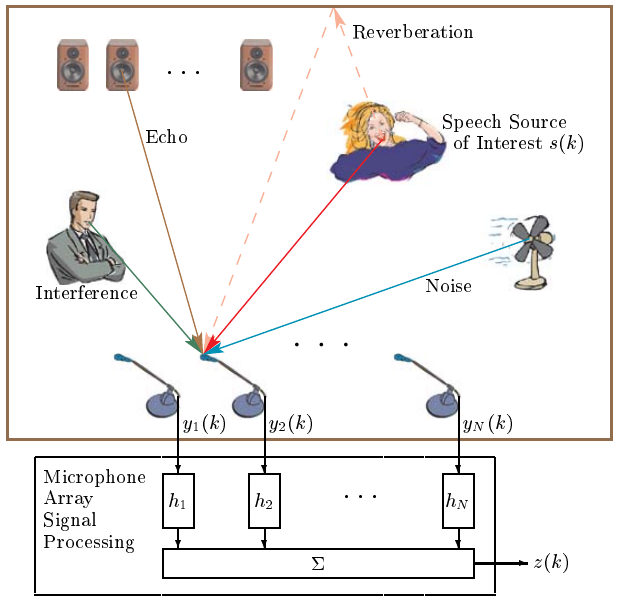
\includegraphics[width=0.65\linewidth]{Beamformers/images/mic_array_proc.png}
    \caption{Microphone array processing}\label{fig:mic_array_proc}
\end{figure}

The coefficients for a DAS beamformer are chosen such that:
\begin{equation}
    \mathbf{W}(j\omega) = \frac{1}{M} \mathbf{A}(j\omega)
\end{equation}

Where \(M\) is a calculated weight given to each coefficient, and
\(\mathbf{A}\) is the steering vector that points 
to the same direction as the direction of arrival.

\subsection{MVDR -- Minimum Variance Distortionless Response}
Another type of beamformer is the MVDR beamformer.
These beamformers aim to minimize the 
sampled variance at the beamformer's output. 
Modeling a microphone array, we can write the propagation of sound 
in the form of:
\begin{align}
    r_{_{1}}(t) &= s(t-D_{_{1}}) + n_{_{1}}(t) \nonumber \\
    r_{_{2}}(t) &= s(t-D_{_{2}}) + n_{_{2}}(t) \nonumber \\
    & \vdots  \nonumber \\
    r_{_{m}}(t) &= s(t-D_{_{m}}) + n_{_{m}}(t)
\end{align}

Where \(r_{_{m}}\) models the absorbed signals by microphone
\(m\), \(s\) stands for the desired speech and \(n\) 
marks all the other artifacts that are considered noise. 
The lagging time \(D_{_{m}}\) corresponds to the room impulse
response \(h_{_{m}}\). Therefore, we can write 
the model for absorbed propagation sound as:
\begin{equation}\label{eq:mic_disc}
    r_{_{m}}[n] = h_{_{m}}[n]\star s[n] + n_{_{m}}[n]
\end{equation}
Transforming Equation\;\ref{eq:mic_disc} to frequency domain,
we get:
\begin{equation}\label{eq:mic_disc}
    \mathbf{R}_{_{m}}(j\omega;t) = \mathbf{H}_{_{m}}(j\omega)\mathbf{S}(j\omega;t) + \mathbf{N}_{_{m}}(j\omega;t)
\end{equation}

MVDR works on minimizing the variance at the 
output resulting from the summation of the 
speech and noise variations at the inputs. 
Therefore, we need a notation for the variances 
and covariances to model the MVDR beamformer. 

Equation\;\ref{eq:mvdr_cov} shows the covariance matrices of the
speech, noise, and the extracted room impulse response, respectively.
\begin{align}\label{eq:mvdr_cov}
    \mathbf{R}_{_{SS}} &= \frac{1}{T}\sum_{t=1}^{T}\mathbf{S}(j\omega;t)\mathbf{S}^{\acute{H}}(j\omega;t) \nonumber \\
    \mathbf{R}_{_{NN}} &= \frac{1}{T}\sum_{t=1}^{T}\mathbf{N}(j\omega;t)\mathbf{N}^{\acute{H}}(j\omega;t)\nonumber \\
    \mathbf{R}_{_{HH}} &= \frac{1}{T}\sum_{t=1}^{T}\mathbf{H}(j\omega)\mathbf{H}^{\acute{H}}(j\omega)|\mathbf{S}(j\omega;t)|^{2} 
\end{align}

Hence, an MVDR beamformers coefficients can be selected following:
\begin{align}
    \displaystyle\mathbf{W}(j\omega) = \frac{\mathbf{R}_{XX}^{-1}(j\omega)\mathbf{A}(j\omega)}{\mathbf{A}^H(j\omega)\mathbf{R}_{XX}^{-1}(j\omega)\mathbf{A}(j\omega)}
\end{align}
Similar to the DAS beamformer, here,
\(\mathbf{A}(j\omega)\) denotes the steering vector.

\subsection{GEV -- Generalized Eigenvalue}
The GEV beamformer is based on the principle of
generalized eigenvalues decomposition so that the beamformer's
coefficients are set accordingly by the extraction of 
the eigenvalue vector \(\lambda\). 
\begin{align}
    \mathbf{R}_{SS}(j\omega)\mathbf{W}(j\omega) = \lambda\mathbf{R}_{NN}(j\omega)\mathbf{W}(j\omega)
\end{align}

GEV beamformers are favorable over MVDR and DAS 
beamformers especially when
the microphone array formation is unknown.
Another case when we should consider a GEV beamformer
is when modeling the steering vector becomes 
a factor due to complex room impulse responses.


% \section{Static Coefficients}

% \section{Dynamic Coefficients}


